\section{INITIAL SHEAR MODULUS AND SHEAR STRENGTH 初始剪切模量和剪切强度}

\begin{paracol}{2}
    
    So far, the authors'effort has been directed toward evaluating relationship between N-value of the standard penetration test and initial shear modulus or shear strength of cohesive soil.
    
    In this section, however, their effort is to be directed solely to evaluating direct relation between initial shear modulus $G_0$ and shear strength $S_u$. It is to be noted here that criteria of data sampling can be more moderate in this section, because of reduction in number of data on initial shear modulus and N-value, compared with the previous sections.
    
    The data for use in this section are from one of the investigations made in the past by other researchers\citet{Shima19681301, Shima1969819} and such data sources as Kajima Institute of Construction Technology by which the authors are employed, involving 20 sites and 194 data in total.

    \switchcolumn

    到目前为止,作者一直致力于评估标准贯入试验的N值与黏性土的初始剪切模量或剪切强度之间的关系。
            
    然而,在本节中,他们的工作将仅针对评估初始剪切模量$G_0$与剪切强度$S_u$之间的直接关系。 这里要注意的是,与之前的部分相比,由于初始剪切模量和N值的数据数量减少,本部分中的数据采样标准可能更为温和。
            
    本节中使用的数据来自于其他研究人员\citet{Shima19681301, Shima1969819}过去的一项调查,以及来自作者的鹿岛建设技术研究所等数据源,涉及20个地点,共194个数据。
    
\end{paracol}

\Paragraph{Criteria of Data Sampling 数据采样标准}

\begin{paracol}{2}

    Criteria of Data Sampling Criteria of data sampling was set up so that the following requirements could be met : 
    \begin{enumerate}
        \item Soil has to fall under the category of cohesive soil.
        \item Shear wave velocity has to be measured by way of the well- shooting test.
        \item Values of $G_0$ and $S_u$ have to be those obtained by experiment at the same site and in the same depth. If there exist several values for $S_u$ corresponding number of data should be made availably by combining each value of $S_u$ with the corresponding value of $G_0$.
    \end{enumerate}

    \switchcolumn

    数据采样标准设置数据采样标准是为了满足以下要求:
    \begin{enumerate}
        \item 土体必须属于黏性土体。
        \item 剪切波速度必须通过射井试验来测量。
        \item $G_0$和$S_u$的值必须是在相同的位置和相同的深度通过实验获得的。 如果存在$S_u$的多个值,则应通过将$S_u$的每个值与$G_0$的对应值进行组合来获得对应数量的数据。
    \end{enumerate}
    
\end{paracol}

\Paragraph{Relation between Initial Shear Modulus and Shear Strength 初始剪切模量与剪切强度之间的关系}

\begin{paracol}{2}
    
    Data on initial shear modulus $G_0$ and shear strength $S_u$ are plotted on a logarithmic graph shown in \autoref{figure:14}. On the assumption that as a first approximation equation should be $G_0=aS_u^b$ and taking the data plotted in \autoref{figure:14} into account, the following empirical formula was obtained by calculating a and b by the method of least squares :

    \switchcolumn

    初始剪切模量$G_0$和抗剪强度$S_u$的数据绘制在\cnfigureref{figure:14}所示的对数图上。假设作为第一近似方程式,应为$G_0=aS_u^b$,并考虑\cnfigureref{figure:14}中绘制的数据, 通过最小二乘法计算$a$和$b$得到以下经验公式:

\end{paracol}

\begin{align}
    G_0=516S_u^{1.012}(\rm{kg/cm^2})
    \label{equation:13}
\end{align}

\begin{figure*}[!htb]
    \begin{minipage}[t]{0.44\textwidth}
        \centering
        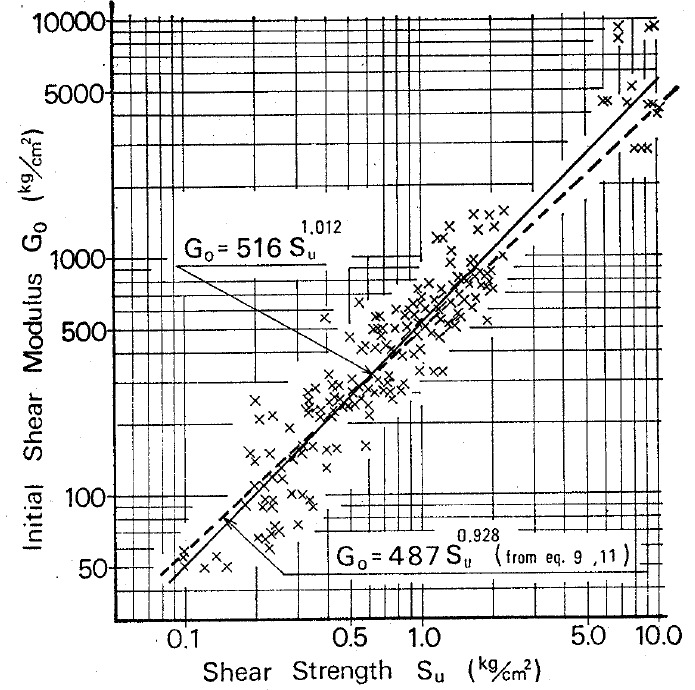
\includegraphics[width=\textwidth]{figures/figure-14.png}
        \caption{Relationship between $G_0$ and $S_u$}
        \addtocounter{figure}{-1}
        \vspace{-5pt}
        \renewcommand{\figurename}{图}
        \caption{$G_0$和$S_u$值之间的关系}
        \renewcommand{\figurename}{Figure}
        \label{figure:14}
    \end{minipage}
    \begin{minipage}[t]{0.52\textwidth}
        \centering
        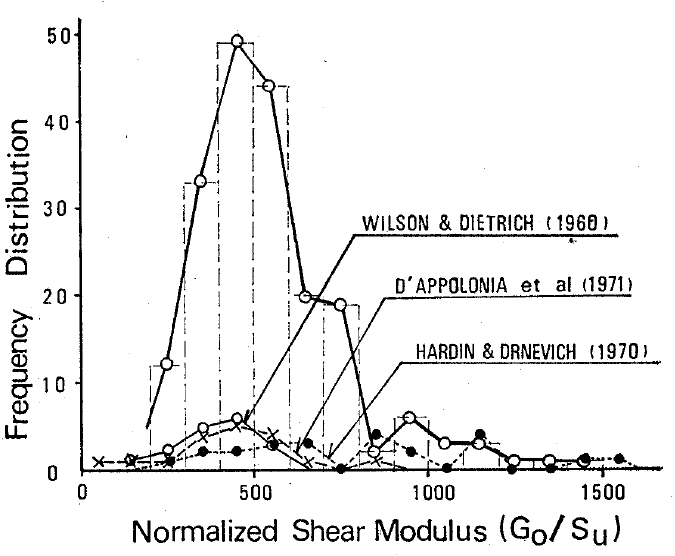
\includegraphics[width=\textwidth]{figures/figure-15.png}
        \caption{Histogram of normalized shear modulus ($G_0/S_u$)}
        \addtocounter{figure}{-1}
        \vspace{-5pt}
        \renewcommand{\figurename}{图}
        \caption{归一化剪切模量的直方图($G_0/S_u$)}
        \renewcommand{\figurename}{Figure}
        \label{figure:15}
    \end{minipage}
\end{figure*}


\begin{paracol}{2}

    \noindent{}where coefficient of correlation $\rho_{xy}=0.95$.

    \switchcolumn
    
    \noindent{}其中相关系数$\rho_{xy}=0.95$。

    \switchcolumn*

    Exponent of $S_u$ in the \autoref{equation:13} is 1.012 or approximately equal to 1.0. $G_0$ can therefore be considered to be in proportion to $S_u$.

    \switchcolumn

    $S_u$在\cnequationref{equation:13}中的指数为1.012或大约等于1.0。 因此,可以认为$G_0$与$S_u$成比例。

\end{paracol}

\Paragraph{Investigation of Normalized Shear Modulus 归一化剪切模量的研究}

\begin{paracol}{2}
    
    Now that $G_0$ is confirmed to be in proportion to $S_u$, it is convenient to define the normalized shear modulus $G_n$ as follows :

    \switchcolumn

    既然已确定$G_0$与$S_u$成比例,则可以方便地将归一化剪切模量$G_n$定义如下:

\end{paracol}

\begin{align}
    G_n=\frac{G_0}{S_u}
    \label{equation:14}
\end{align}

\begin{paracol}{2}
    
    \autoref{figure:14} shows a histogram of the normalized shear modulus drawn by calculating values of $G_n$ from the data plotted in \autoref{figure:14}. The value of $G_n$ are in the region ranging from 250 to 1430, with the mean value of 548 and the standard deviation of 211.
    
    For comparison, the following values of $G_n$ can be quoted independently from the data obtained by \citet{Hardin1973667}, \citet{Wilson2010419} and \citet{DAppolonia19711359}.

    \switchcolumn

    \cnfigureref{figure:15}显示了通过从\cnfigureref{figure:14}中绘制的数据计算$G_n$值得出的归一化剪切模量的直方图。$G_n$值在250到1430的范围内,平均值为548,标准偏差为211。
    
    为了比较,可以独立于由\citet{Hardin1973667},\citet{Wilson2010419}和\citet{DAppolonia19711359}获得的数据引用的以下$G_n$值。

    \switchcolumn*
    
    \begin{enumerate}
        \item \citet{Hardin1973667} have obtained the initial shear modulus and the shear strength of the same cohesive soil by means of a reasonant-column apparatus in the laboratory. The normalized shear modulus $G_n$ calculated from these values is ranging from 380 to 1500 with its mean value of about 760.
        \item \citet{Wilson2010419} have obtained the values of initial Young's modulus, initial shear modulus and compressible strength by measuring a -longitudinal or torsional natural frequency of clay samples. The value of $G_n$ can be calculated from these measured data by assumming the Poisson's ratio as 0.5, and it is in the region ranging from 178 to 550 with its mean value of about 390.
        \item \citet{DAppolonia19711359} have shown eleven combinations of data on the initial Young's modulus and the shear strength by in-situ and laboratory tests. 
    \end{enumerate}      

    \switchcolumn
    
    \begin{enumerate}         
        \item \citet{Hardin1973667}通过实验室中的推理柱设备获得了同一粘性土的初始剪切模量和剪切强度。 根据这些值计算出的归一化剪切模量$G_n$介于380至1500之间,其平均值约为760。
        \item \citet{Wilson2010419}通过测量黏土样品的纵向或扭转自然频率获得了初始杨氏模量,初始剪切模量和可压缩强度的值。 可以通过将泊松比设为0.5来从这些测量数据中计算出$G_n$值,该值处于178至550范围内,平均值约为390。
        \item \citet{DAppolonia19711359}通过现场和实验室测试,已显示出有关初始杨氏模量和剪切强度的11种数据组合。
    \end{enumerate}

    \switchcolumn*
    
    The value of $G_n$ calculated from these values by assumming the Poisson's ratio as 0.5 is in the region ranging from 53 to 833 with its mean value about 420. 
    
    The results of these investigations are shown in \autoref{figure:15} for comparison with the authors' result. The histogram in \autoref{figure:15} shows that the peaks of frequency distribution curves are in the region ranging from 400 to 500 except \citet{Hardin1973667}'s data.

    \switchcolumn
       
    通过假设泊松比为0.5,从这些值计算出的$G_n$值在53到833范围内,其平均值约为420。
       
    这些研究的结果如\cnfigureref{figure:15}所示,以便与作者进行比较。\cnfigureref{figure:15}的直方图显示,除\citet{Hardin1973667}的数据外,频率分布曲线的峰值在400到500范围内。
    
\end{paracol}